
\begin{figure}[t]
   \centering
   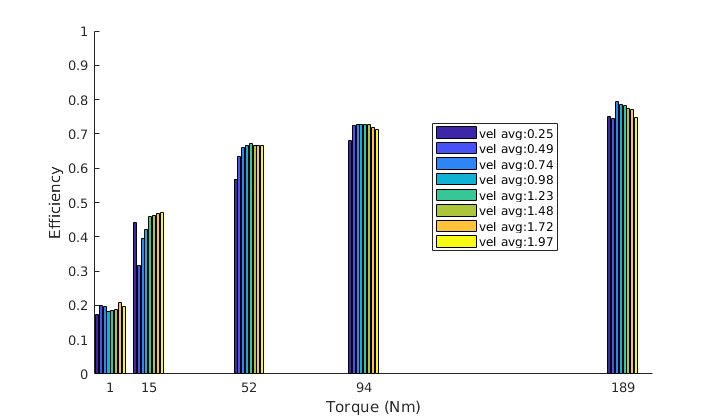
\includegraphics[width=\linewidth]{images/eff_test_bar_plot_v2}
   \caption{Grouping of average efficiencies at each torque step.
   Efficiency depends heavily on torque, and slightly on speed.}
   \label{eff_results}
\end{figure}

Duty cycle testing was first performed on the actuator.
These tests were done at lower torques to prevent the motor from overheating to allow extended duration testing.
The total test time prior to these duty cycle tests was approximately 5.2 hours to bring up and check out the actuator testbed system.
Once this checkout was complete, the 100 hours of duty cycle testing were conducted the course of 11 days with the drive cycle discussed in Section \ref{methods}.
Three of the torque/speed combinations in forward and reverse are plotted on Fig \ref{long_run} to show the general characteristic trends seen in actuator performance.

After this duty cycle testing to ensure the actuator had sufficiently broken-in and achieved steady state performance, the pure efficiency cycles were run.
As discussed in Section \ref{methods}, a profile of speeds and torques were run on the actuator to show the relationship between speed, torque, and efficiency.
An example of this profile can be seen in Fig \ref{eff_profile}.
This profile was run three times and the results at each torque and speed combination were averaged (see Fig \ref{eff_results}.
